\documentclass[aspectratio=169, table]{beamer}

%\usepackage[beamertheme=./praditatheme]{Pradita}
\usepackage[utf8]{inputenc}
\usepackage{xcolor} % for color
\usepackage{colortbl} % for table color
\usepackage{listings}


% Tambahkan ini di preamble jika belum ada
\usepackage{tcolorbox} % untuk kontrol warna border block

% Tambahkan ini sebelum \begin{document} atau di awal frame
	\colorlet{blockborder}{gray!40}
	\setbeamercolor{block title}{bg=white, fg=black}
	\setbeamercolor{block body}{bg=white, fg=black}

% Define Java language style for listings
\lstdefinestyle{JavaStyle}{
language=Java,
basicstyle=\ttfamily\scriptsize,
keywordstyle=\color{blue},
commentstyle=\color{gray},
stringstyle=\color{red},
breaklines=true,
showstringspaces=false,
tabsize=2,
captionpos=b,
numbers=left,
numberstyle=\tiny\color{gray},
frame=lines,
backgroundcolor=\color{lightgray!10},
comment=[l]{//},
morecomment=[s]{/*}{*/},
commentstyle=\color{gray}\ttfamily,
string=[s]{'}{'},
morestring=[s]{"}{"},
%	stringstyle=\color{teal}\ttfamily,
%	showstringspaces=false
}

\usetheme{Pradita}
%
\subtitle{Virtual/Augmented Reality Seminar}

\title{\LARGE{User Experience for\\Virtual/Augmented Reality\\\vspace{10pt}}}
\date[Serial]{\scriptsize {Tangerang, 20th May 2025 }}
\author[Pradita]{\small {\textbf{Alfa Yohannis}}}

\begin{document}

\frame{\titlepage}

\begin{frame}[fragile]
\frametitle{Contents}
\vspace{20pt}
\begin{columns}[t]
\column{0.5\textwidth}
\tableofcontents[sections={1-5}]

\column{0.5\textwidth}
\tableofcontents[sections={6-10}]
\end{columns}
\end{frame}


\section{Virtual/Augmented Reality}
\begin{frame}{Virtual/Augmented Reality}
	\vspace{20pt}
	
	
	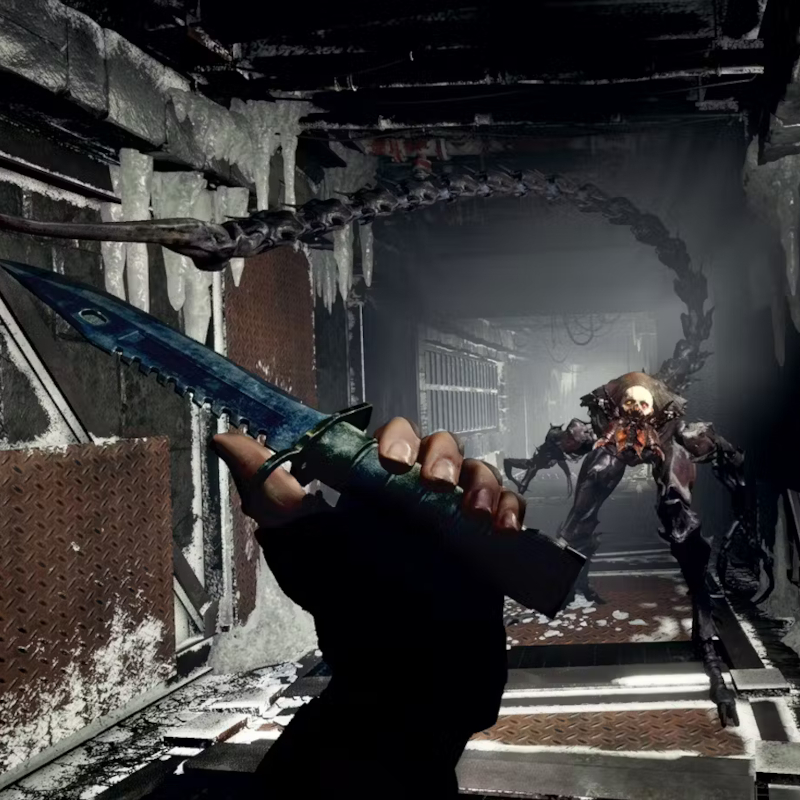
\includegraphics[width=0.246\textwidth, keepaspectratio=true]{../figures/resident_evil.jpg}
	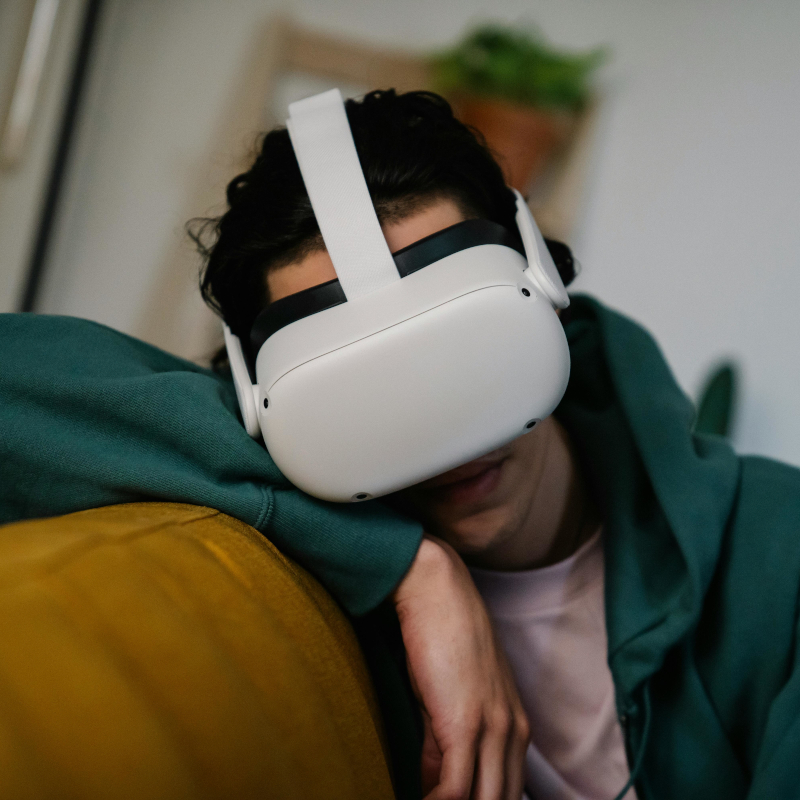
\includegraphics[width=0.246\textwidth,  keepaspectratio=true]{../figures/oculus.jpg} 
	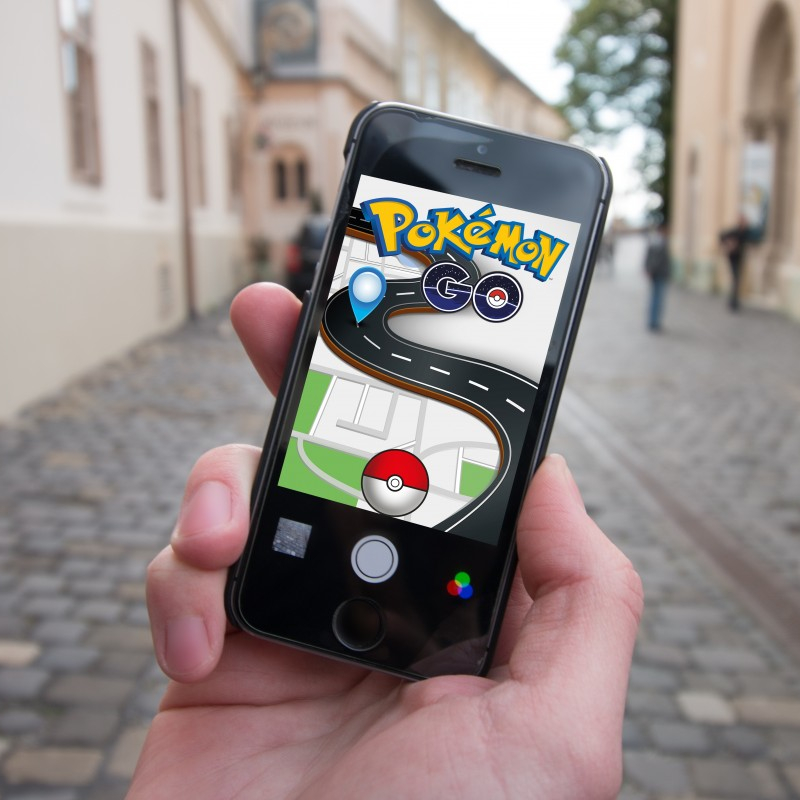
\includegraphics[width=0.246\textwidth, keepaspectratio=true]{../figures/pokemon.jpg} 
	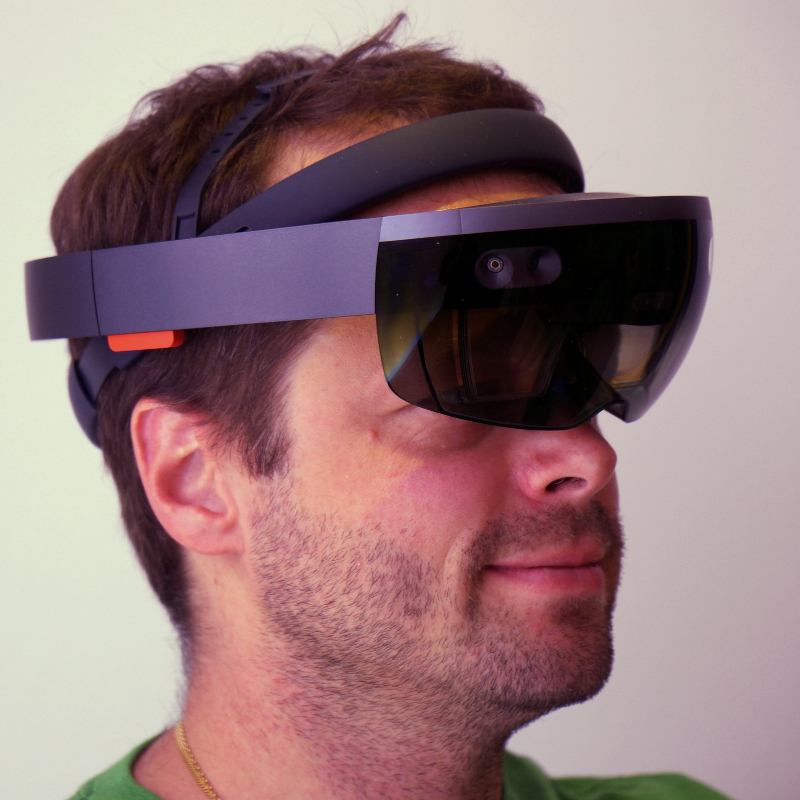
\includegraphics[width=0.246\textwidth,  keepaspectratio=true]{../figures/hololens.jpg}
	
%	\vspace{10pt}
	\vspace{10pt}
	\textbf{Virtual Reality (VR)} and \textbf{Augmented Reality (AR)} change how users interact with digital content. These technologies introduce \textbf{spatial, physical, and sensory dimensions} to user interaction — moving beyond traditional screen-based UX.
	
	\vspace{10pt}
	\centering
	\large
	\textbf{Does anyone know the main difference between the two?}
%	\vspace{5pt}
%	\begin{itemize}
%		\item \textbf{VR (Virtual Reality)} creates a fully immersive digital world. 		
%		\item \textbf{AR (Augmented Reality)} overlays virtual elements onto the real world.
%	\end{itemize}
\end{frame}


\section{What is User Experience (UX)?}

\begin{frame}{What is User Experience (UX)?}
	\vspace{8pt}
	
	\begin{tikzpicture}[remember picture, overlay]
		\node[anchor=north west, inner sep=0pt] at ([xshift=.82\textwidth, yshift=-.01\textwidth] current page.north west){
			
\includegraphics[width=.27\paperwidth]{../figures/frustated_user.jpg} 
		};
	\node[anchor=north west, inner sep=0pt] at ([xshift=.82\textwidth, yshift=-.32\textwidth] current page.north west){
		
\includegraphics[width=.27\paperwidth]{../figures/happy_user.jpg} 
	};
	\end{tikzpicture}
	
	
	\begin{columns}[T]
		\begin{column}{0.7\textwidth}
			User Experience (UX) refers to how users \textbf{feel} when interacting with a system. It covers aspects such as:
			
			\vspace{5pt}
			\begin{itemize}
				\item \textbf{Usability} – How easy and intuitive it is to use
				\item \textbf{Accessibility} – Can all users use it, including those with limitations?
				\item \textbf{Efficiency} – How fast can users achieve their goals?
				\item \textbf{Satisfaction} – Do users enjoy the interaction?
			\end{itemize}
			
			\vspace{5pt}
			Traditional UX applies mostly to \textbf{2D interfaces} like websites or mobile apps. VR/AR introduces new UX challenges in a \textbf{3D spatial context}.
			
			\vspace{8pt}
			\centering
			\large
			\textbf{What are the challenges?}
		\end{column}
		\begin{column}{0.2\textwidth}
		\end{column}
	\end{columns}
	
\end{frame}

\section{Why UX in VR/AR is Different}
\begin{frame}{Why UX in VR/AR is Different}
	\vspace{20pt}
	UX design for immersive environments introduces new dimensions beyond screen-based interaction.
	
	\vspace{5pt}
	\begin{center}
		\arrayrulecolor{gray!60} % Set border color to dark gray
		
		\begin{tabular}{|p{4cm}|p{6cm}|}
			\hline
			\rowcolor{gray!10}
			\textbf{Traditional UX} & \textbf{VR/AR UX} \\
			\hline
			2D interface (screen) & 3D spatial environment \\
			\hline
			Mouse / touch input & Motion controller / hand / gesture \\
			\hline
			Static viewport & Head-tracked dynamic viewpoint \\
			\hline
			Click and scroll & Move, grab, rotate, walk \\
			\hline
			UI overlays & Context-aware spatial UI \\
			\hline
		\end{tabular}
		
		\arrayrulecolor{black} % Reset border color
	\end{center}
	
	\vspace{5pt}
	In VR/AR, the user is \textit{inside} the interface — this requires rethinking usability, interaction flow, and comfort.
	
	\vspace{5pt}
	\centering
	\large
	\textbf{Could you identify any other differences?}
\end{frame}

\section{Common UX Challenges in VR/AR}
\begin{frame}{Common UX Challenges in VR/AR}
	\vspace{20pt}
	Immersive environments introduce specific UX challenges:
	
	\vspace{5pt}
	\begin{itemize}
		\item \textbf{Motion Sickness} – Caused by mismatch between visual motion and body perception.
		\item \textbf{Navigation Difficulty} – Users may feel lost in large virtual spaces.
		\item \textbf{Complex Interactions} – Grabbing or pointing can feel unnatural without feedback.
		\item \textbf{Visual Overload} – Too much info in 360° views can overwhelm users.
		\item \textbf{Physical Fatigue} – Long sessions with gestures or head movement cause tiredness.
	\end{itemize}
	
	\vspace{5pt}
	UX design in VR/AR must address both physical and mental demands.
	
	\vspace{5pt}
	\centering
	\large
	\textbf{Have you ever experienced any of these challenges?\\How did you feel at that time?}
\end{frame}


\section{Good UX Practices for VR/AR}

\begin{frame}{Good UX Practices for VR/AR}
	\vspace{20pt}
	To create comfortable and effective VR/AR experiences, designers should follow these key practices:
	
	\vspace{5pt}
	\begin{itemize}
		\item \textbf{Simplify interactions} – Use intuitive hand gestures and avoid complex controls.
		\item \textbf{Support spatial orientation} – Provide visual anchors and minimize disorientation.
		\item \textbf{Limit unnecessary motion} – Reduce user movement to avoid fatigue and nausea.
		\item \textbf{Provide consistent feedback} – Use visual, haptic, or audio cues for actions.
		\item \textbf{Design for comfort} – Consider user posture, session length, and accessibility.
	\end{itemize}
	
	\vspace{5pt}
	Immersive UX should feel natural, predictable, and non-intrusive.
	
	\vspace{5pt}
	\centering
	\large
	\textbf{Which of these practices do you think is most critical?\\What would you add based on your own experience?}
\end{frame}



\section{Case Study – Beat Saber}
\begin{frame}{Case Study – Beat Saber}
	\vspace{5pt}
	
		\begin{tikzpicture}[remember picture, overlay]
		\node[anchor=north west, inner sep=0pt] at ([xshift=.82\textwidth, yshift=-.2\textwidth] current page.north west){
			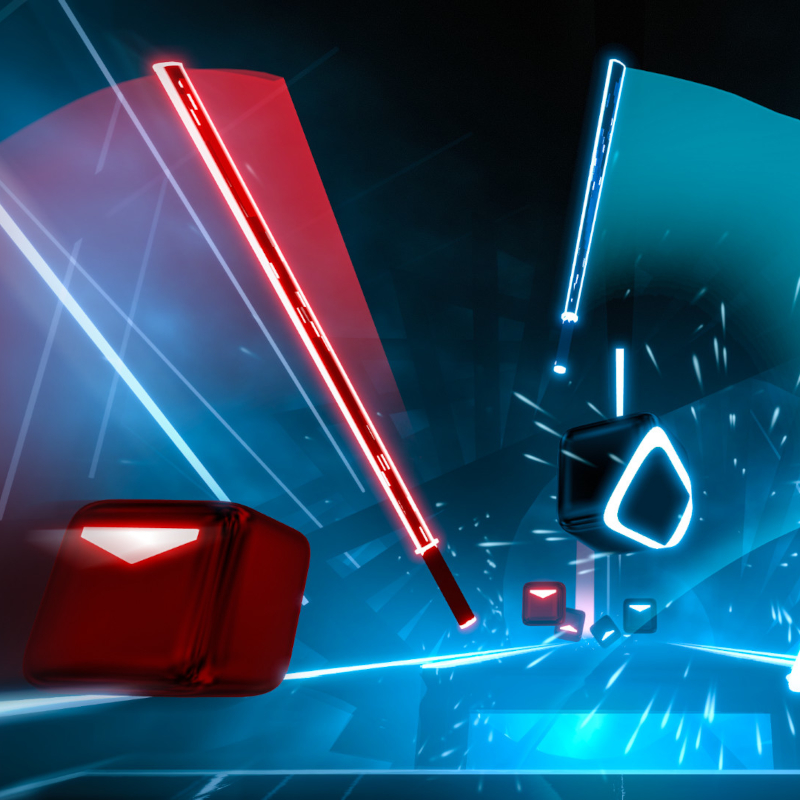
\includegraphics[width=.27\paperwidth]{../figures/beat_saber.jpg} 
		};
	\end{tikzpicture}
	
	\begin{columns}[T]
		\begin{column}{0.75\textwidth}
			\textbf{Why is Beat Saber a good example of VR UX?}
			
			\vspace{5pt}
			\begin{itemize}
				\item \textbf{Simple Controls} – Slice blocks using two hand-held sabers with intuitive motion.
				\item \textbf{Clear Feedback} – Immediate visual and audio responses on success or failure.
				\item \textbf{Static Positioning} – User stays in one spot, reducing motion sickness.
				\item \textbf{Minimal Interface} – No cluttered UI elements during gameplay.
				\item \textbf{Rhythm-based Design} – Naturally encourages user focus and flow.
			\end{itemize}
			
		\end{column}
		\begin{column}{0.2\textwidth}
		\end{column}
	\end{columns}

				\vspace{10pt}
\small \textbf{Beat Saber shows how good UX can make VR experiences fun, accessible, and engaging.}
\end{frame}


\section{Quick Example – Bad vs Good UX}
\begin{frame}{Quick Example – Bad vs Good UX}
	\vspace{8pt}
	\begin{columns}[T]
		\column{0.48\textwidth}
		\textbf{Bad UX in VR:}
		\begin{itemize}
			\item No onboarding or tutorial
			\item Cluttered interface blocks vision
			\item Awkward hand gestures required
			\item Motion causes dizziness
		\end{itemize}
		
		\column{0.48\textwidth}
		\textbf{Good UX in VR:}
		\begin{itemize}
			\item Clear onboarding and guidance
			\item Minimal, floating UI elements
			\item Natural and consistent gestures
			\item Static user position avoids sickness
		\end{itemize}
	\end{columns}
	
	\vspace{20pt}
	\centering
	\textbf{\large{A good VR experience makes users feel in control, not confused or exhausted.}}
\end{frame}


	\section{Activity / Discussion}
	\begin{frame}{Activity / Discussion}
		\vspace{10pt}
		\textbf{Quick Question for You:}
		
		\vspace{8pt}
		\begin{tcolorbox}[colframe=blockborder, colback=gray!05, coltitle=black, title=\textbf{What would frustrate you most in a VR classroom app?}]
			\begin{itemize}
				\item Too much unnecessary movement?
				\item Hard-to-use controls?
				\item UI blocking your field of view?
				\item Confusing spatial layout?
			\end{itemize}
		\end{tcolorbox}
		
		\vspace{10pt}
		\textbf{Follow-up:} \\
		What features would you design to make it feel \textit{comfortable and usable}?
		
		\vspace{6pt}
		\small (Discuss with a partner or share an answer aloud)
	\end{frame}

\section{Summary}
\begin{frame}{Summary}
	\vspace{10pt}
	\textbf{Key Takeaways:}
	
	\vspace{8pt}
	\begin{itemize}
		\item UX in VR/AR requires \textbf{rethinking traditional design rules}.
		\item Users are immersed — not just viewing a screen, but \textit{inside} the interface.
		\item Good design reduces motion sickness, fatigue, and confusion.
		\item Successful UX feels \textbf{intuitive, spatially aware, and comfortable}.
	\end{itemize}
	
	\vspace{10pt}
	\textbf{Final Thought:} \\
	Design for humans first — the tech comes second.
\end{frame}


\end{document}
                                                                                                                                                                               